\documentclass[a4paper,12pt]{article} % добавить leqno в [] для нумерации слева
\usepackage[a4paper,top=1.3cm,bottom=2cm,left=1.5cm,right=1.5cm,marginparwidth=0.75cm]{geometry}
%%% Работа с русским языком
\usepackage{cmap}					% поиск в PDF
\usepackage{mathtext} 				% русские буквы в фомулах
\usepackage[T2A]{fontenc}			% кодировка
\usepackage[utf8]{inputenc}			% кодировка исходного текста
\usepackage[english,russian]{babel}	% локализация и переносы

\usepackage{graphicx}

\usepackage{wrapfig}
\usepackage{tabularx}

\usepackage{hyperref}
\usepackage[rgb]{xcolor}
\hypersetup{
colorlinks=true,urlcolor=blue
}
\usepackage{multirow}
\usepackage{hhline}


%%% Дополнительная работа с математикой
\usepackage{amsmath,amsfonts,amssymb,amsthm,mathtools} % AMS
\usepackage{icomma} % "Умная" запятая: $0,2$ --- число, $0, 2$ --- перечисление

%% Номера формул
\mathtoolsset{showonlyrefs=true} % Показывать номера только у тех формул, на которые есть \eqref{} в тексте.

%% Шрифты
\usepackage{euscript}	 % Шрифт Евклид
\usepackage{mathrsfs} % Красивый матшрифт

%% Свои команды
\DeclareMathOperator{\sgn}{\mathop{sgn}}

%% Перенос знаков в формулах (по Львовскому)
\newcommand*{\hm}[1]{#1\nobreak\discretionary{}
{\hbox{$\mathsurround=0pt #1$}}{}}

\begin{document}

\newenvironment{lines}[1][\textwidth] % по умолчанию линейки на всю ширину текста
{
\newcolumntype{E}{>{}p{#1}<{\hrulefill}} % в конце нашего столбца будет приписываться \hrulefill
\begin{flushright} % автоматически вставим flushright
\begin{tabular}[h]{E} % и tabular нужного формата
}
{\end{tabular}\end{flushright}
}
	
	\begin{titlepage}
	\begin{center}
		{\large МОСКОВСКИЙ ФИЗИКО-ТЕХНИЧЕСКИЙ ИНСТИТУТ (НАЦИОНАЛЬНЫЙ ИССЛЕДОВАТЕЛЬСКИЙ УНИВЕРСИТЕТ)}
	\end{center}
	\begin{center}
		{\large Физтех-школа электроники, фотоники и молекулярной физики}
	\end{center}
	
	
	\vspace{4.5cm}
	{\huge
		\begin{center}
			{Лабораторная работа 5.7.1}\\
			Измерение углового распределения жесткой компоненты космического излучения
		\end{center}
	}
	\vspace{2cm}
	\begin{flushright}
		{\LARGE Салтыкова Дарья \\
			\vspace{0.5cm}
			Б04-105}
	\end{flushright}
	
	\vspace{0.5cm}
	
	\begin{lines}[.5
	\textwidth]
  {\LARGE Допуск} \rule{6.5cm}{0.25pt} \vspace{0.5cm}\\
 {\LARGE Выполнение} \rule{3cm}{0.25pt}\vspace{0.5cm} \\ {\LARGE Сдача} \rule{3cm}{0.25pt} \\ % \rule сделает линейку указанной длины и толщины
\end{lines}
	\vspace{6cm}
	\begin{center}
		Долгопрудный 2023
	\end{center}
\end{titlepage}

\section{Введение}

\noindent
\textbf{Цель работы:} с помощью телескопа и двух сцинтилляторов измеряется угловое распределение жесткой компоненты космического излучения и на основе полученных данных оценивается время жизни мюона.

\section{Теоретические сведения}

\noindent Космические лучи --- это стабильные частицы и ядра атомов, зародившиеся и ускоренные до больших энергий вне Земли, изотропно падающие на границу земной атмосферы (первичное космическое излучение), а также различные частицы, рожденные ими при взаимодействии с ядрами атомов воздуха (вторичное космическое излучение).

\medskip
	
\noindent Первичное космическое излучение --- протоны($90\%$) и $\alpha$ частицы ($10\%$). Для протонов сечение взаимодействия с ядрами атомов, содержащихся в воздухе, близко к геометрическому и равняется 	
	$$\sigma_{p \ air} \simeq \pi R^2 = \pi (R_0 A^{\frac1{3}}) = 300\text{мб}$$
	
\noindent Тогда слой атмосферы при таких сечениях есть $8\div 12$ свободных пробегов протонов.
	
\medskip	
	
\noindent Вторичные частицы включают в себя пионы, каоны и гипероны. Для пиона время жизни $\tau_0 = 2,5\cdot 10^{-8}$ и схема распада
	$$\pi^{\pm} \rightarrow \mu^{\pm} + \nu$$
	
\noindent Но также возможно взаимодействие с ядрами атомов воздуха. Какое из двух событий произойдет зависит от плотности атмосферы. Пробег для распада:	
	$$L_{\text{расп}} = \beta c \tau_0 \gamma = \frac{c\tau_0 E_\pi}{m_\pi c^2}$$
		
		
\noindent А для взаимодействия:
	$$L_{\text{вз}} = \frac1{\sigma_{\pi\ air} n} = \frac{A} {\sigma_{\pi\ air} \rho N}, \ \sigma_{\pi\ air}\simeq \frac2{3} \sigma_{p \ air} \simeq 200 \text{мб} $$
	
\noindent Тогда вероятность взаимодействия равна вероятности распада при
	$$ E_\pi =  \frac{A m_\pi c^2} {\sigma_{\pi\ air} \rho N c \tau_0}$$
	
\noindent Мюоны же преимущественно вызывают ионизацию воздуха. Для прохождения всей атмосферы энергия должна составлять порядка $2$ГэВ. Распад мюона происходит со временем жизни $\tau_0 = 2\cdot 10^{-6}$ по каналам:
	$$\mu^{+} \rightarrow e^+ + \widetilde{\nu_e} + \nu_\mu, \ \mu^{-} \rightarrow e^- + \widetilde{\nu_\mu} + \nu_e$$
	
\noindent Время жизни увеличивается $\tau = \tau_0 \gamma$. При этом распадный пробег мюона с энергией $2$ГэВ есть 
	$$L_{\text{расп}} = \beta c \tau_0 \gamma \approx 12km$$
	
\noindent Также в сильных взаимодействиях рождаются нейтральные пионы, распадающиеся на два гамма-кванта. Их время жизни мало и они не успевают взаимодействовать с атомными ядрами. Гамма кванты же в поле атомных ядер рождают электрон-позитронные пары.
	
\medskip	
	
\noindent Процесс продолжается лавинообразно и один нейтральный пион может дать начало лавине, число частиц в которой достигает $10^5$.  Как следтсвие одна частица с энергией $10^{20}$эВ дает на уровне моря лавину с числом частиц порядка $10^{10}.$
	
\noindent Исследования показывают, что интенсивность распределения космических лучей резко зависит от направления, увеличиваясь при переходе к вертикальному. При этом по вертикали мюоны проходят порядка $L_0 \simeq 15km$. Тогда 
	$$\Delta L = L_0(\frac1{\cos \theta} - 1)$$
	$$P(\Delta L) = 1 - \exp(-\Delta L / L_\text{расп}), L_\text{расп} = c\tau$$
	
\noindent А также число дошедших мюонов уменьшается за счет поглощения в веществе по закону
	$$P_1(\theta) \propto (\cos\theta)^{1,6}$$
	
\noindent А из-за распада мюонов
	$$P_2(\theta) = \exp(-L(\theta)/L)$$
	
\noindent Тогда отношение числа мюонов, идущих под зенитным углом $\theta$, к числу вертикально падающих есть
	$$\frac{N(\theta)}{N(0)} =  \frac{P_1(\theta)P_2(\theta)}{P_1(0)P_2(0)} = (\cos\theta)^{1,6} \frac{e^{-L(\theta)/L}}{e^{-L(0)/L}}$$
	
\noindent Учитывая $L(\theta) = L_0 / \cos\theta$, получаем оценку на время жизни $\tau_0$.
		
	
	\section{Экспериментальная установка}
	
	
	
\noindent Установка регистрирует те частицы, которые летят внутри обозначенного телесного угла. Схема регистрирует истинные и случайные совпадения.
	
\medskip	
	
\noindent Число случайных совпадений $N = 2\tau N_1 N_2$, где $N_1, N_2$ --- число импульсов за единицу времени от каждого счетчика.

\medskip
	
\noindent Величину разрешающего времени стараются максимально уменьшить. Для данной геометрии $\tau \simeq (1\div 2) \cdot 10^{-6}$c.
	
	\begin{figure}[h!]
		\centering
		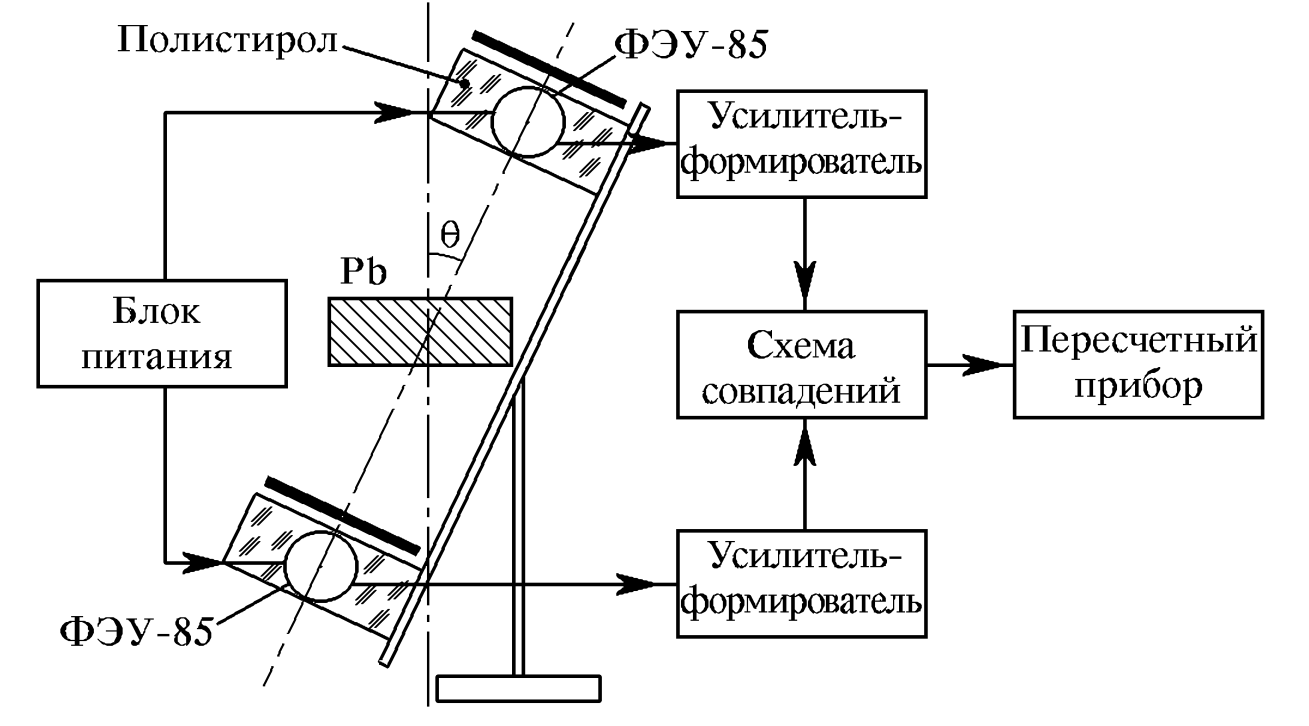
\includegraphics[width=0.8\linewidth]{kosmos.png}
		\caption{Экспериментальная установка}
	\end{figure}
	
\newpage
	
\section{Ход работы}

\noindent 1. Проведем оценку фонового излучения.

$$I_\text{ф} = 0,081 \pm 0,004, ( \varepsilon = 5 \%)$$

\noindent 2. \textbf{Определим толщину свинцового фильтра}, который следует установить между счетчиками телескопа, чтобы регистрировать только жесткую компоненту космического излучения.

\medskip

\noindent Измерим зависимость скорости счета N от толщины поглотителя x. I - частота двойных совпадений I* с учетом фона и случайных совпадений (см. ниже).

\begin{table}[h!]
\begin{tabular}{|c|l|l|l|l|}
\hline
\multicolumn{1}{|l|}{$t, \text{c}$} & $N$ & $x, \text{мм}$ & $I^*, \text{1/с}$ & $I, \text{1/с}$ \\ \hline
\multirow{6}{*}{600}                & 378 & 2              & 0,630            & 0,549           \\ \cline{2-5} 
                                    & 366 & 4              & 0,610            & 0,529           \\ \cline{2-5} 
                                    & 357 & 12             & 0,595            & 0,514           \\ \cline{2-5} 
                                    & 354 & 20             & 0,589            & 0,508           \\ \cline{2-5} 
                                    & 346 & 30             & 0,577            & 0,495           \\ \cline{2-5} 
                                    & 342 & 40             & 0,569            & 0,488           \\ \hline
\end{tabular}
\end{table}

\noindent \textbf{Оценим число случайных совпадений.} 

$$I_{\text{случ}} = 2\tau I_1 I_2 = 2\tau \frac{N_1N_2}{T^2}$$


\noindent Для проведенного эксперимента $\tau = 10^{-7} c$, $T = 300 c$, $N_1 = 3328$, $N_2 = 3489$. Отсюда $I_{\text{случ}} \approx 2,4 \cdot 10^{-4} \text{ 1/c}$.

\medskip

\noindent Построим кривую поглощения.

\begin{figure}[h!]
    \centering
    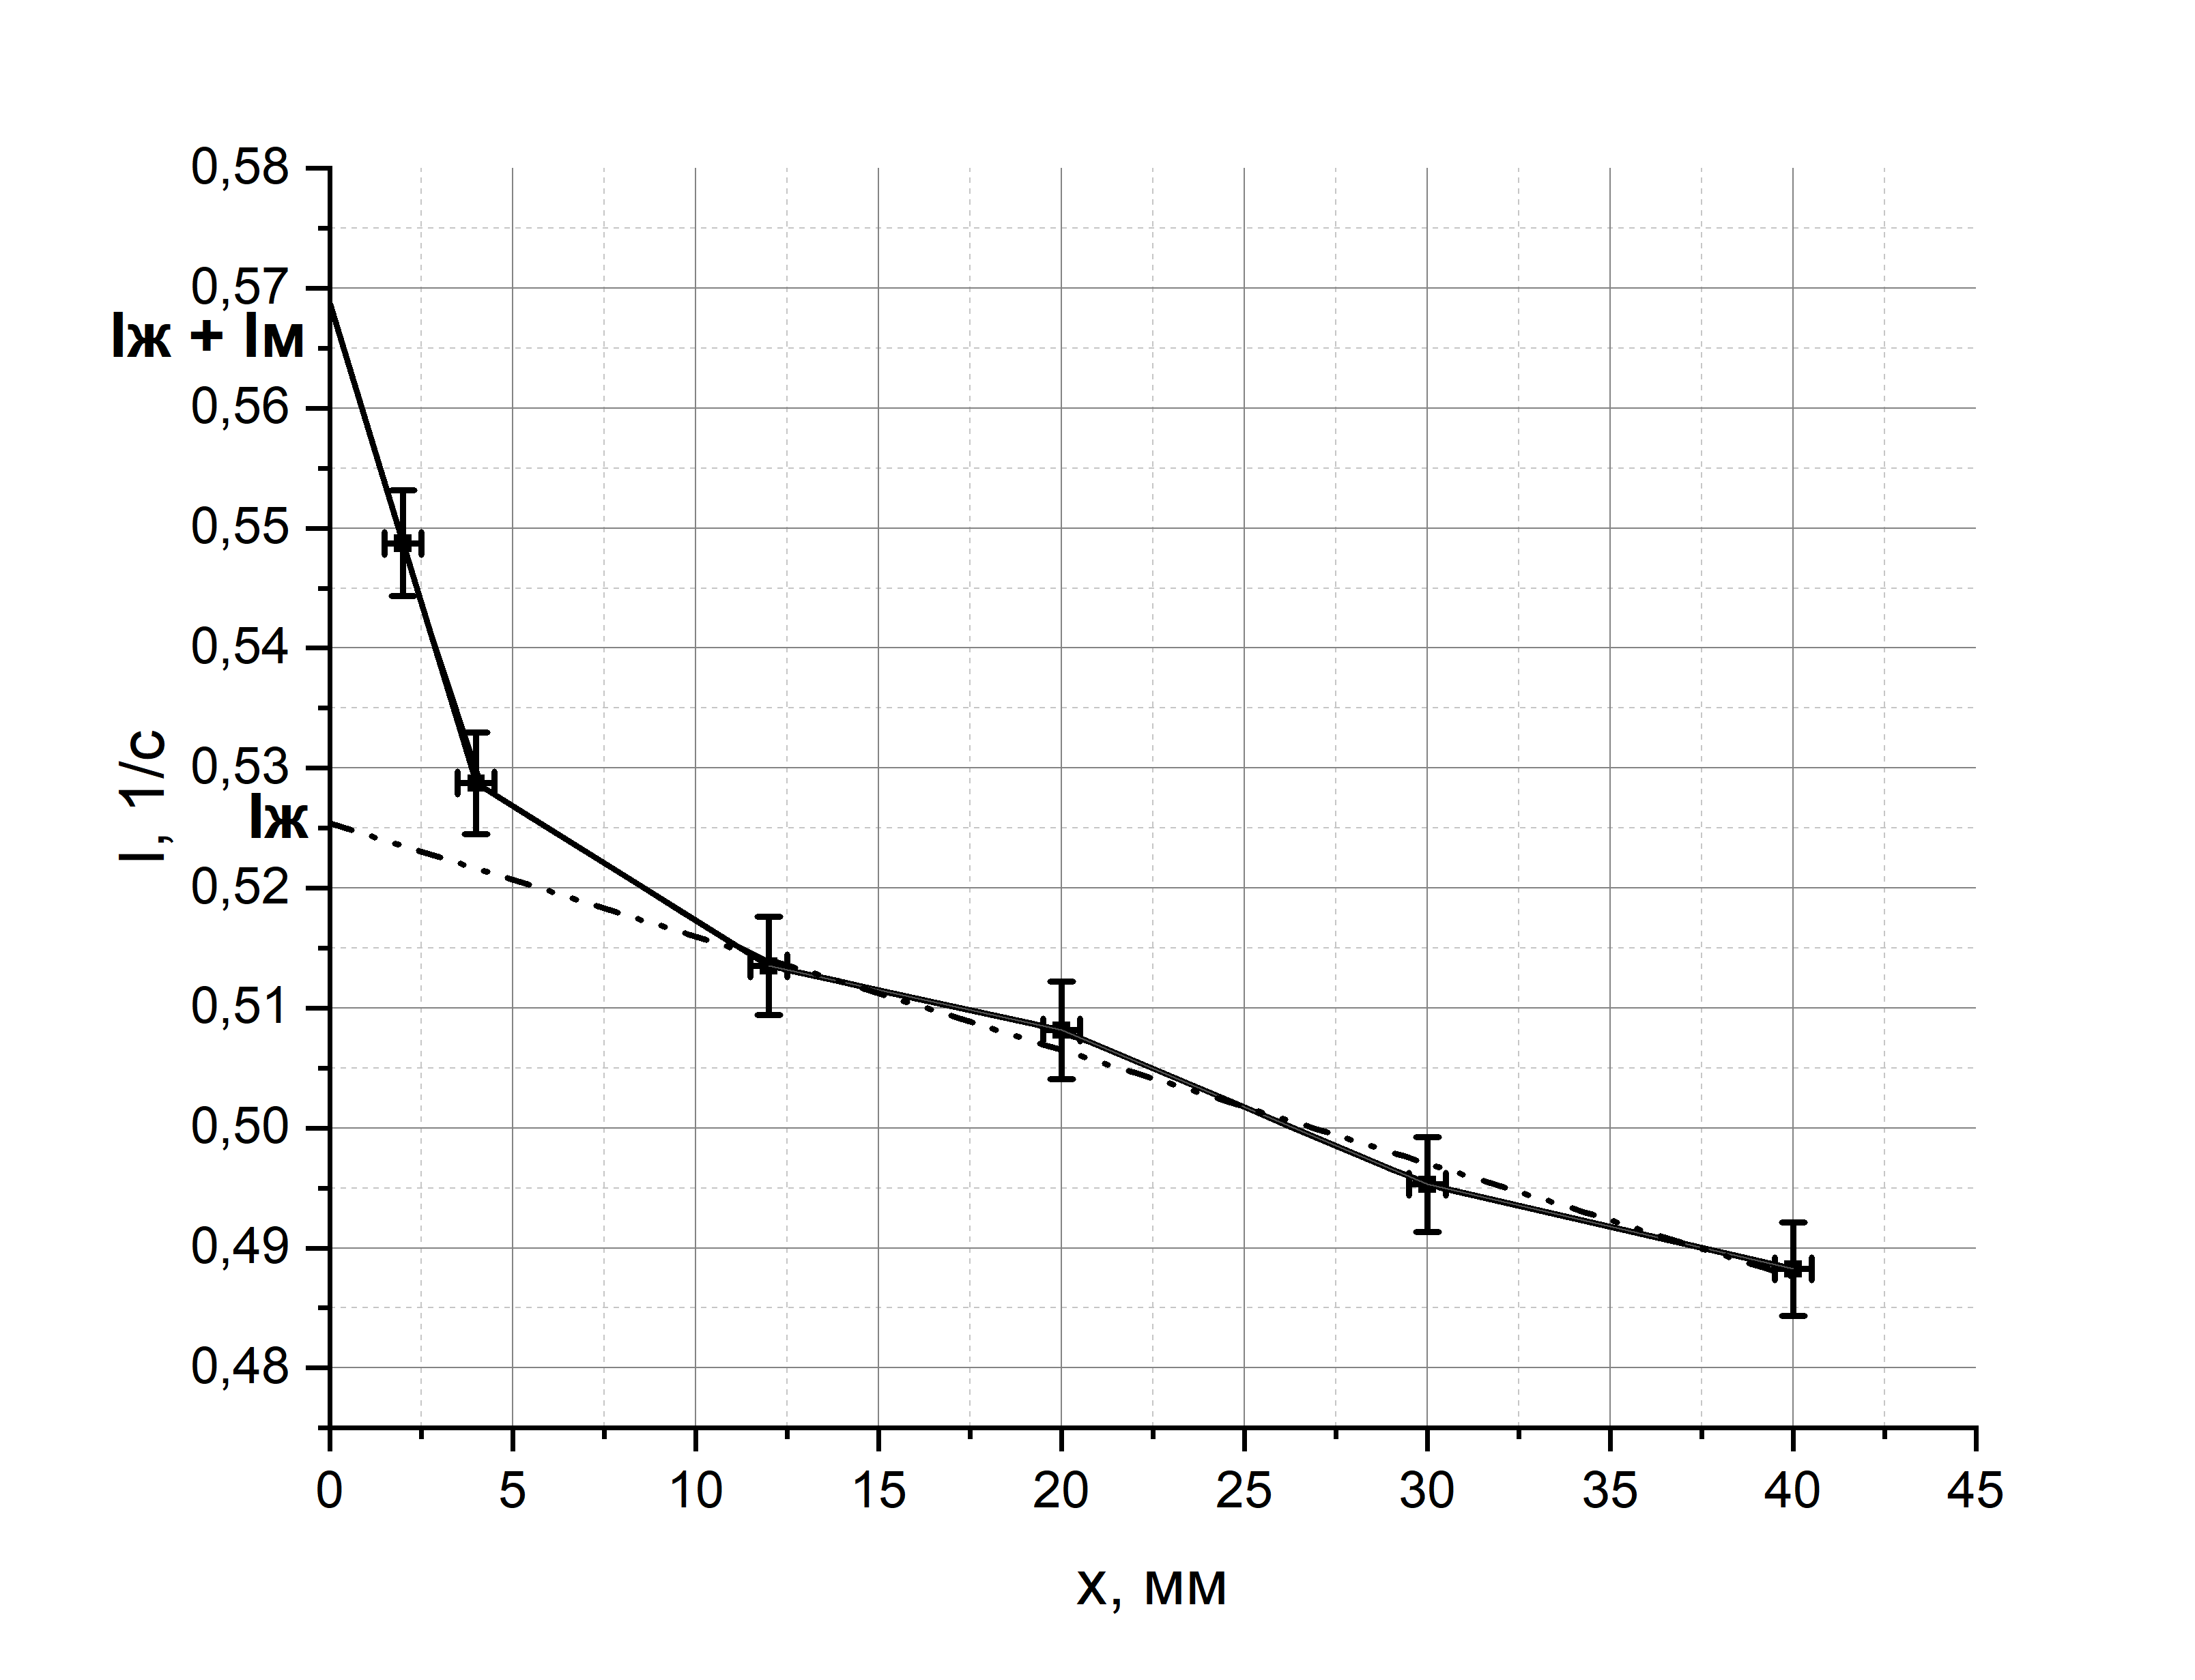
\includegraphics[scale=0.5]{1.png}
    \caption{Кривая поглощения}
    
\end{figure} 

\noindent Определим интенсивность мягкой $I_{\text{м}}$ и жесткой $I_{\text{ж}}$ компонент.

$$I_{\text{м}} = (0,0432 \pm 0,0002) \text{ 1/c}$$
$$I_{\text{ж}} = (0,525 \pm 0,002) \text{ 1/c}$$

\noindent 3. \textbf{Изучим угловое распределение жесткой компоненты космических лучей}. Для этого необходимо поместить между детекторами свинцовый фильтр толщиной, выбранной в соответствии с измеренной кривой поглощения. Однако во время выполнения работы выяснилось, что при наличии свинцовых пластин установка не выдерживает поворот на нужный угол, поэтому измерения проводились без них. Таким образом, отсеивание мягкой компоненты произведено не было.

\medskip

\noindent Измерим угловую зависимость интенсивности излучения I в диапазоне от 0 до 70 градусов.

\begin{table}[h!]
\begin{tabular}{|c|l|l|l|l|l|l|l|}
\hline
\multicolumn{1}{|l|}{$t, \text{c}$} & $\theta, ^\circ$ & $ln(cos \theta)$ & $N$ & $I^*, \text{1/c}$ & $I, \text{1/с}$ & $I/I_0$ & $ln(I/I_0)$ \\ \hline
\multirow{5}{*}{600}                & 0                & 0                & 528 & 0,880             & 0,799           & 1       & 0           \\ \cline{2-8} 
                                    & 20               & -0,062           & 424 & 0,706             & 0,625           & 0,783   & -0,245      \\ \cline{2-8} 
                                    & 30               & -0,144           & 396 & 0,660             & 0,579           & 0,725   & -0,322      \\ \cline{2-8} 
                                    & 50               & -0,442           & 312 & 0,520             & 0,439           & 0,550   & -0,598      \\ \cline{2-8} 
                                    & 70               & -1,073           & 248 & 0,413             & 0,332           & 0,415   & -0,879      \\ \hline
\end{tabular}
\end{table}

\noindent Построим график зависимости $lnI$ от $ln cos \theta$. 

\begin{figure}[h!]
    \centering
    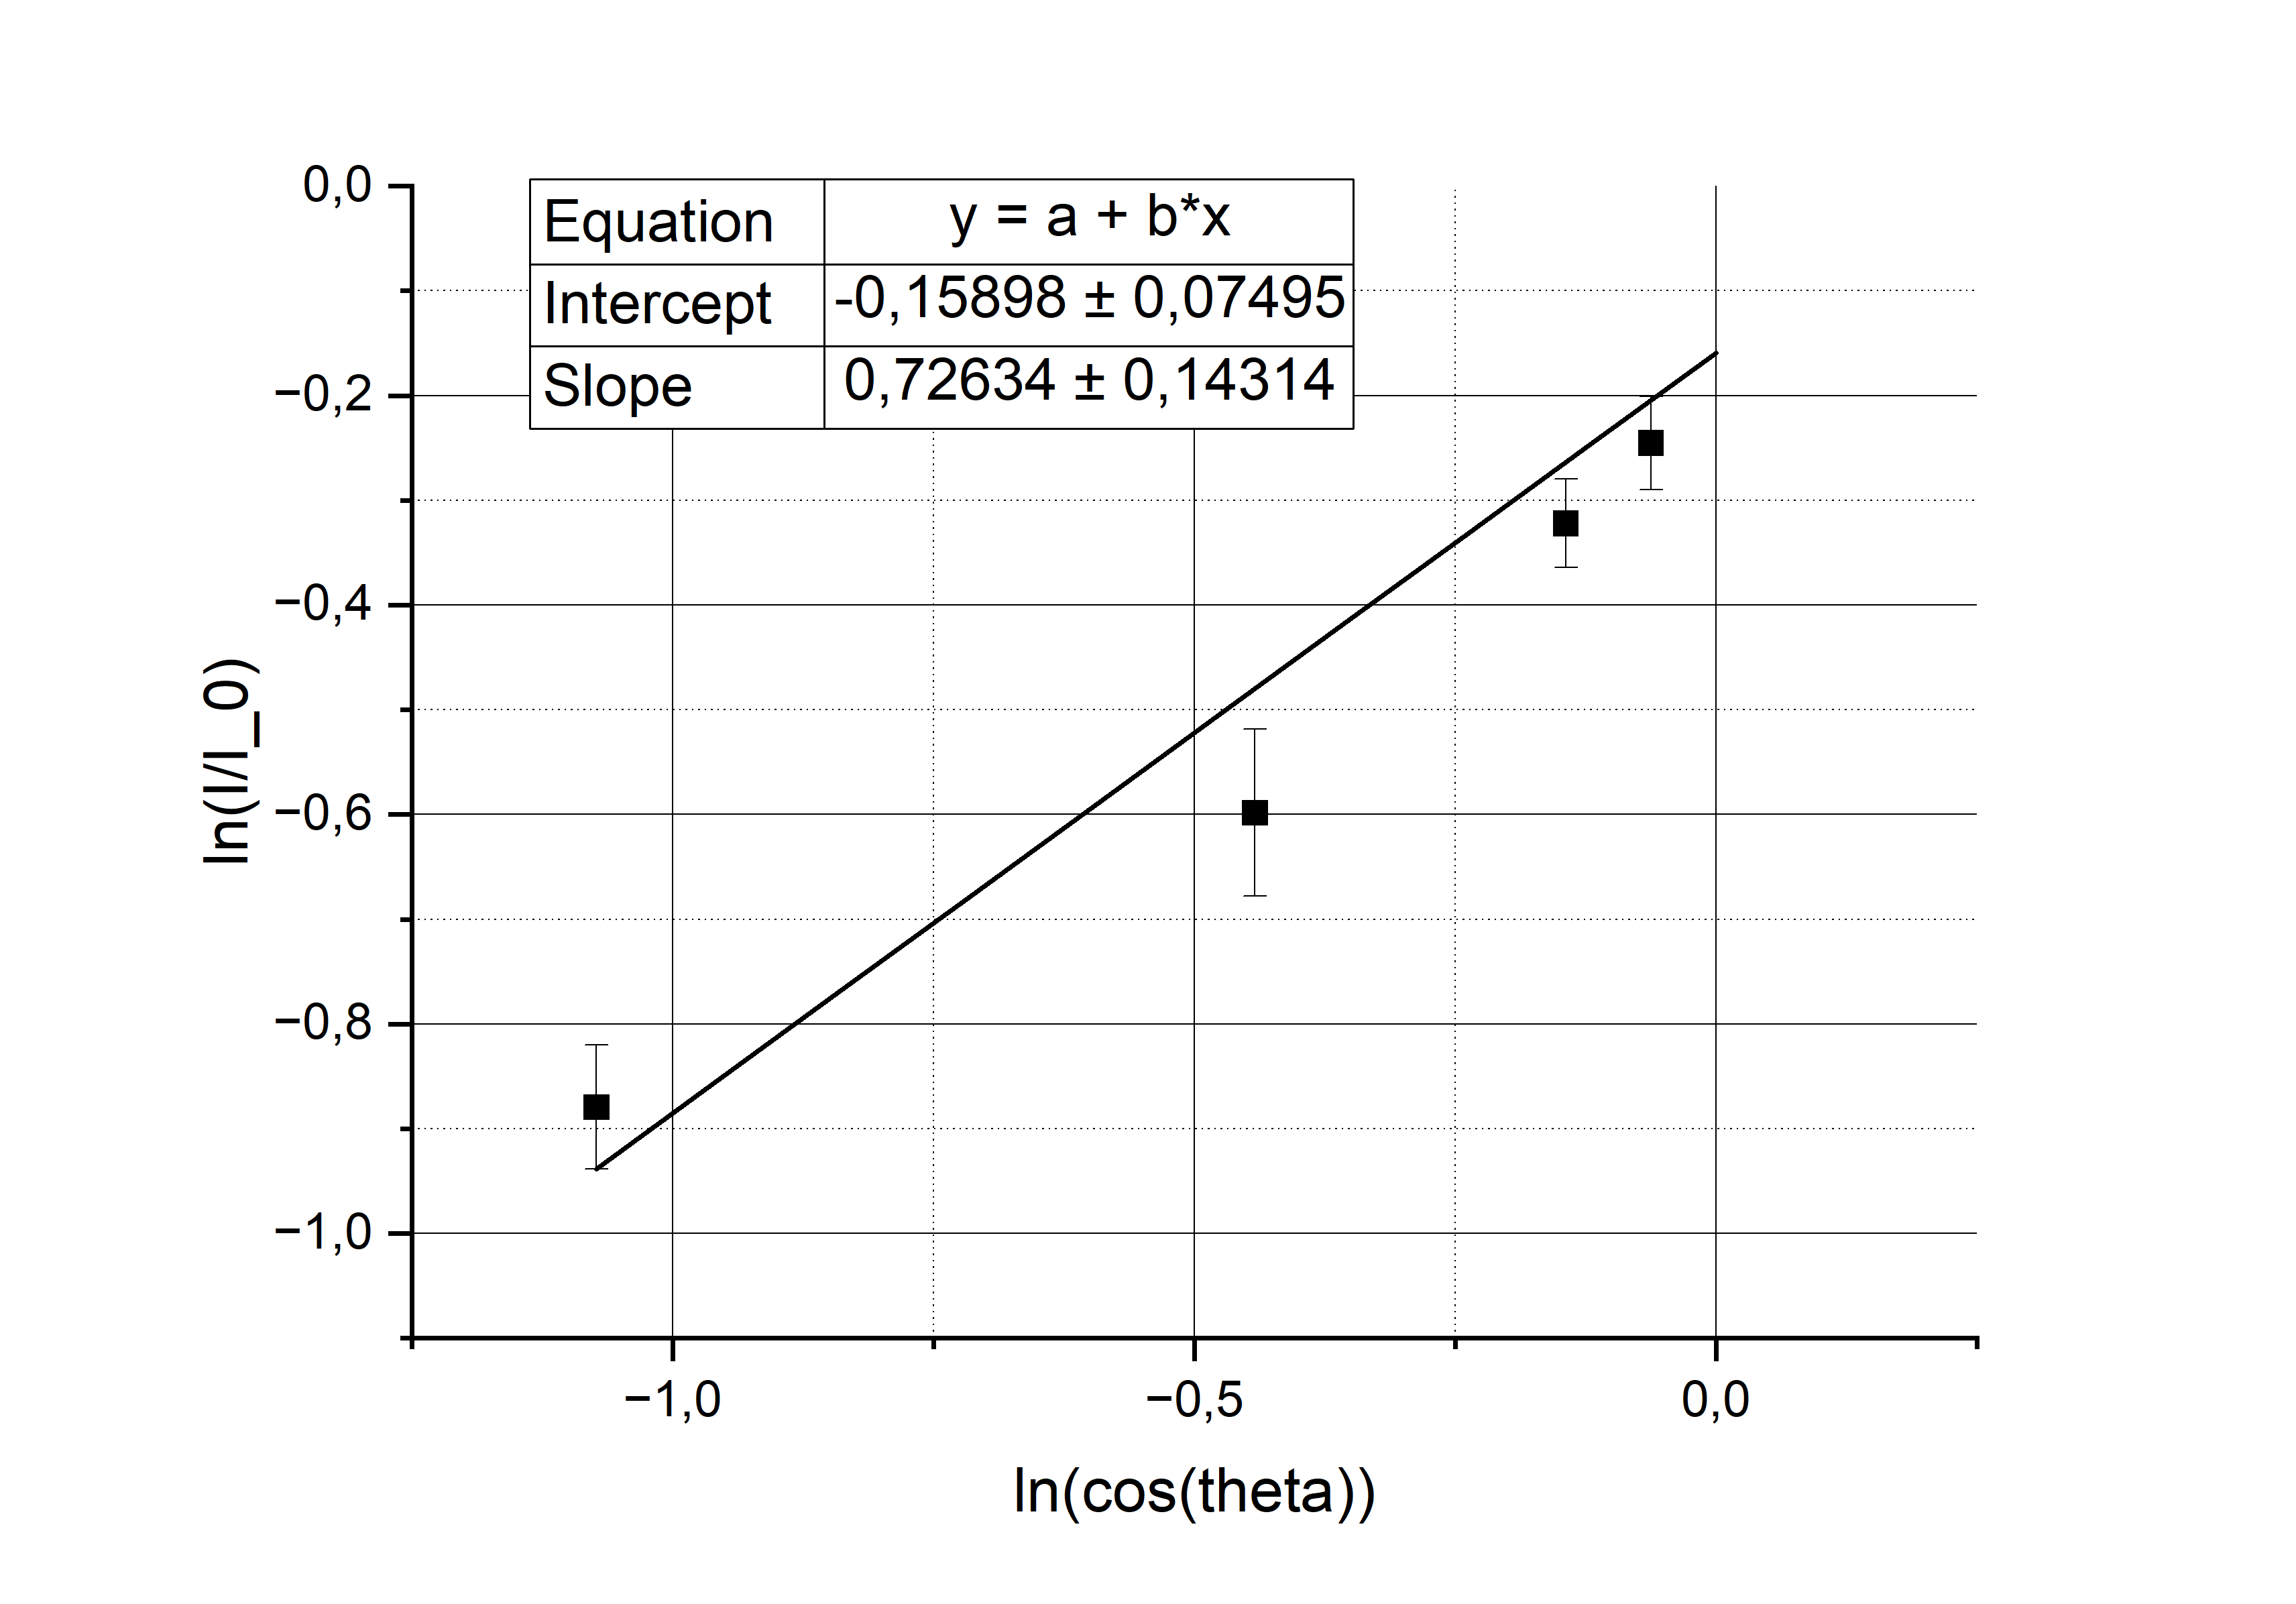
\includegraphics[scale=0.5]{2.png}
    \caption{$ln(I/I_0) (ln cos \theta)$}
    
\end{figure}

\noindent \textbf{Определим показатель экспоненты n в угловой зависимости $I = I_0 cos^n \theta$}. $n = 0,72 \pm 0,14.$

\medskip

\noindent \textbf{Оценим время жизни мюона.} Из графика (для $\theta = 50^{\circ}$): $\frac{I(\theta)}{I(0)} = 0,619 $.

\medskip

\noindent Из теории время жизни мюона:

$$\tau_0 = \dfrac{L_0 (\cos\theta - 1)}{\cos\theta (\ln\frac{N(\theta)}{N(0)} - 1,6\ln\cos \theta)} \cdot \dfrac {m_\mu c^2}	{\beta c E_\mu}.$$
	
\noindent Учитывая табличные значения полной энергии, энергии покоя и величины свободного пробега мюона. 

$$\tau_0 = 1,05 \pm 0,12 \text{ мкс}\ ( \varepsilon = 9\% )$$

\section{Вывод}

\noindent В ходе работы было проведено измерение угловой зависимости интенсивности космического излучения (без исключения мягкой компоненты) и оценено время жизни мюона.

\medskip

\noindent По кривой поглощения были определены интенсивности мягкой и жесткой компонент космического излучения $I_{\text{м}} = (0,0432 \pm 0,0002) \text{ 1/c}$, $I_{\text{ж}} = (0,525 \pm 0,002) \text{ 1/c}$.

\medskip

\noindent Также был получен показатель $n = 0,72 \pm 0,14$ теоретически предсказанной зависимости $I = I_0 \cos^n\theta$. Значение не совпадает с теоретическим $n_{\text{теор}} = 1,6$, вероятно, из-за влияния мягкой компоненты. 

\medskip
	
\noindent На последнем этапе работы было оценено время жизни мюона: $\tau_0 = 1,05 \pm 0,12 \text{ мкс}$. Табличное значение $\tau_{0_{\text{теор}}} = 2,2 \text{ мкс}.$ Проведенные расчеты дают значение $\tau_0$ только по порядку величины, поскольку они не учитывают как меняется вероятность распада мюонов из-за уменьшения их энергии вследствие ионизационного торможения.

\end{document}